\section{Problem (4)}

	In the \cref{fig:hw4_problem4}, a stone is projected at a cliff of height $h$ with an initial speed of $39 \ m/s$ directed at an angle $\theta_{0} = 66^{o}$ above the horizontal. The stone strikes at $A$, $4.1 \ s$ after launching.

	\begin{figure}[H]
		\begin{center}
			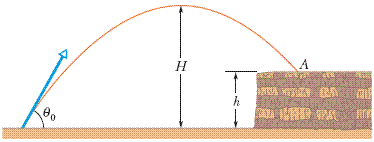
\includegraphics[scale=1]{hw4_problem4}
			\caption{Illustration of Problem 4}
			\label{fig:hw4_problem4}
		\end{center}
	\end{figure}

	\subsection{Question (a)}
		Find the height $h$ of the cliff:

		\textbf{R:} \newline
		\begin{align}
			y = \ &y_{0} + v_{0_{y}}t + \frac{1}{2}a_{y}t^{2}& \notag \\
			y = \ &h& \notag \\
			v_{0_{y}} = \ &v_{0} \sin 66^{o}& \notag \\
			= \ &(39 \ m/s)(0.9135) = 35.6265 \ m/s& \notag \\
			h = \ &(35.6265 \ m/s)(4.1 \ s) + \left(-4.9 \ m/s^{2}\right)(4.1 \ s)^{2}& \notag \\
			= \ &(150.1687 \ m) - (82.3690 \ m)& \notag \\
			= \ &67.7997 \ m&
		\end{align}

	\subsection{Question (b)}
		Find the speed of the stone just before impact at $A$:

		\textbf{R:} \newline

		\begin{align}
			v_{x} = \ &v_{0_{x}} + a_{x}t = v_{0_{x}}& \notag \\
			v_{x} = \ &v_{0} \cos 66^{o}& \notag \\
			= \ &(39 \ m/s)(0.4067) = 15.8613 \ m/s& \notag \\
			v_{y} = \ &v_{0_{y}} + a_{y}t& \notag \\
			= \ &(35.6265 \ m/s) + \left( -9.8 \ m/s^{2} \right)(4.1 \ s)& \notag \\
			= \ &(35.6265 \ m/s) - (40.1800 \ m/s) = - 4.5535 \ m/s& \notag \\
			\left| \vec{v} \right| = &\sqrt{(15.8613 \ m/s)^{2} + (-4.5535 \ m/s)^{2}}& \notag \\
			= &16.5020 \ m/s&
		\end{align}

	\subsection{Question (c)}
		Find the maximum height $H$ reached above the ground.

		\textbf{R:} \newline
		\begin{align}
			v_{y} = \ &v_{0_{y}} + a_{x}t& \notag \\
			0 = \ &(35.6265 \ m/s) + \left( -9.8 \ m/s^{2} \right)t& \notag \\
			t = \ &\frac{-35.6265 \ m/s}{-9.8 \ m/s^{2}} = 3.6354 \ s& \notag \\
			y = \ &y_{0} + v_{0_{y}}t + \frac{1}{2}a_{y}t^{2}& \notag \\
			y = \ &H& \notag \\
			H = \ &(35.6265 \ m/s)(3.6354 \ s) + \left(-4.9 \ m/s^{2}\right)(3.6354 \ s)^{2}& \notag \\
			= \ &(133.1520 \ m) - (64.7591 \ m)& \notag \\
			= \ &68.3929 \ m&
		\end{align}
